\chapter{\texorpdfstring{Development and Validation of an mpMRI-anchored
CT{} Habitat
Model}{Development and Validation of an mpMRI-anchored CT Habitat Model}}\label{development-and-validation-of-an-mpmri-anchored-ct-habitat-model}

In Chapter 6, we identified a set of precise handcrafted radiomics
features for stable CT{} habitat computation. An exploratory analysis
suggested qualitative agreement between these habitats and histologic
phenotypes such as necrosis and viable cancer. In this chapter, we
address the central question arising from that observation: can CT{}
habitats capture the tissue phenotypes that dominate colorectal liver
metastases?

The key methodological strength is the use of the PREDICT dataset (see
Section 5.1.). Each CT{} voxel is paired with aligned mpMRI maps
reflecting cellularity and vascularity. This allows us to evaluate CT{}
habitats against pseudo-biological ground truth during development---not
just post-hoc.

\textbf{Contributions:}

\begin{itemize}
\item
  We compare four CT{} data representations for habitat
  computation---raw Hounsfield units, handcrafted radiomics features,
  deep learning features from a liver tumor segmentation model, and deep
  learning features from a foundation model---and identify the
  representation that yields the most biologically coherent habitats.
\end{itemize}

\begin{itemize}
\item
  We develop an mpMRI-anchored framework for CT{} habitat discovery,
  using co-registered multiparametric MRI as a surrogate for tissue
  cellularity and vascularity.
\end{itemize}

\begin{itemize}
\item
  We validate CT{} habitats against whole-tumor histopathology
  annotations of necrosis, fibrosis, and viable cancer in resected
  samples.
\end{itemize}

The work presented in Chapters 7 and 8 forms the basis of a manuscript
currently in preparation.

\section{Rationale}\label{rationale-1}

Colorectal cancer is the third most common malignancy worldwide, and the
liver is its most frequent site of metastasis (Arnold et al., 2017;
Siegel, Miller, et al., 2020). Approximately half of patients with
colorectal cancer will develop liver metastases during their disease
course. While surgical resection offers the best change for long-term
survival, the majority of patients present with unresectable disease and
receive systemic therapy (i.e. chemotherapy and/or targeted therapy).
Response to these therapies is highly variable, and a significant
proportion of patients develop resistance (Zeineddine et al., 2023).

Tumor heterogeneity is increasingly recognized as a driver of this
resistance. Colorectal liver metastases are not uniform masses but
histologically complex ecosystems containing variable proportions of
viable tumor, necrosis, and fibrosis. These compartments carry
prognostic significance: fibrosis often indicates favorable response to
chemotherapy (Poultsides et al., 2012), while central necrosis may
reflect treatment failure due to poor drug penetration (Wong \& Neville,
2007b). If we could distinguish these tissue states non-invasively, we
might stratify patients more accurately and guide treatment decisions
earlier.

Habitat imaging offers a potential solution. By clustering voxels into
spatially distinct subregions, habitats can identify tissue compartments
that correspond to different biological states, potentially including
necrosis, fibrosis and viable cancer. In Chapter 6, we demonstrated that
stable CT{} habitats can be computed using a precise subset of
handcrafted radiomics features, and we observed qualitative
correspondence with histologic phenotypes in an exploratory analysis.
Two questions remained open: Can CT{} habitats reliably capture these
three dominant tissue phenotypes? And if so, are handcrafted features
the optimal CT{} representation for this task?

This second question arises from the fact that deep learning has
transformed medical image analysis over the past decade. Radiology
foundation models have become recently available and encode rich
hierarchical information after being trained on extremely alrge
datasets. In conventional radiomics studies (i.e. bulk radiomics, not
voxelwise studies) several studies have compared handcrafted and deep
learning features for outcome prediction. For habitat imaging, however,
no study has compared these representations. Thus, to date, we do not
know whether the representational capacity of deep learning trnaslated
into more biologically coherent habitats, or if simpler handcrafted
features are enough.

Answering these questions requires a reference standard that captures
tissue biology at the voxel level. Histopathology is the gold standard
for tissue characterization, but voxel-to-pixel alignment between
radiology and pathology remains technically challenging. Tissue deforms
during resection and fixation; the scale mismatch between radiology
slices (\textasciitilde1--2 mm) and histology sections
(\textasciitilde4--5 μm) complicates spatial correspondence; and
registration errors accumulate.

Multiparametric MRI offers a middle ground between
histology\textquotesingle s cellular resolution and
CT{}\textquotesingle s accessibility. Diffusion-weighted imaging (DWI),
the primary non-invasive MRI technique for probing tissue microstructure
(Le Bihan et al., 2001), measures water diffusion at scales far below
the millimeter-level image resolution. In tumors, apparent diffusion
coefficient (ADC) values inversely correlate with cellularity: dense
cellular packing restricts water motion, yielding low ADC (Chen et al.,
2013; Surov et al., 2017). Advanced diffusion models can also estimate
microvascular volume fraction (fv), a marker of tissue vascularity
(Federau et al., 2014; Togao et al., 2018). Similarly, dynamic
contrast-enhanced (DCE) MRI quantifies vascular properties through
pharmacokinetic modeling. Parameters such as the transfer constant
(\emph{Ktrans)} have been validated as markers of tumor vascularity and
perfusion (Jackson et al., 2007; Tofts \& Kermode, 1991). Together,
these modalities provide voxel-level maps of biologically meaningful
tissue states---cellularity and vascularity---that are impractical to
obtain from histology alone. If CT{} habitats reflect true biology, they
should naturally differentiate tissue according to these same underlying
properties.

The PREDICT cohort provides a unique resource since patients underwent
both contrast-enhanced CT{} and multiparametric MRI. This enables
something beyond post-hoc validation---it allows us to select the CT{}
representation whose habitats best align with mpMRI-derived biophysical
metrics. Rather than computing CT{} habitats and hoping they reflect
biology, we can ask directly: which CT{} features produce clusters that
separate tissue with different cellularity and vascularity? The
resulting model is not merely validated against mpMRI; it is anchored to
it. mpMRI serves as both the selection criterion and the biological
reference.

We followed a two-stage strategy. First, in the PREDICT cohort, we
compared four CT{} representations and selected the one whose habitats
best separated mpMRI-derived measures of cellularity (ADC) and
vascularity (fv, Ktrans). Second, we applied the selected model to the
POEM cohort---patients with resected colorectal liver metastases and
whole-tumor histopathology---to confirm that habitats exhibit spatial
organization consistent with necrotic cores, fibrotic regions, and
viable tumor rims.

Our hypothesis was that CT{} habitats can capture the three dominant
histological phenotypes of colorectal liver metastases: necrosis,
fibrosis, and viable tumor. We tested this by identifying the optimal
CT{} representation, characterizing the biological profile of each
habitat using mpMRI, and validating the spatial correspondence against
whole-tumor histopathology.

\section{Methods}\label{methods-1}

\subsection{Study Design and Patient Cohorts}\label{study-design-and-patient-cohorts}

This study employed two cohorts to develop, characterize, and validate
the CT{} habitat model (\hyperref[_Ref219844810]{Figure 7.1}).

\begin{quote}
\textbf{1. CT}{} \textbf{Habitat Model Development and Characterization
(PREDICT).} The PREDICT cohort (Section 5.1.2) comprises patients with
colorectal liver metastases who underwent both contrast-enhanced CT{}
and multiparametric MRI before treatment. CT{} was acquired in the
portal venous phase; mpMRI included T2-weighted, diffusion-weighted, and
dynamic contrast-enhanced sequences. Quantitative mpMRI maps---including
ADCt, Ktrans, and fv---were derived as described in Section 5.1.2. For
the present analysis, we included 10 patients (42 tumors) with evaluable
imaging on both modalities and successful CT{}--mpMRI co-registration.

\textbf{2. Histopathological Validation (POEM).} The POEM cohort
(Section 5.1.3) was used for independent validation against biological
ground truth. This cohort includes 6 patients with colorectal liver
metastases who underwent surgical resection. Whole-tumor specimens were
processed for histology and annotated for necrosis, fibrosis, and viable
tumor, providing a macroscopic spatial reference for validating habitat
architecture.
\end{quote}

\begin{figure}[htbp]
\centering
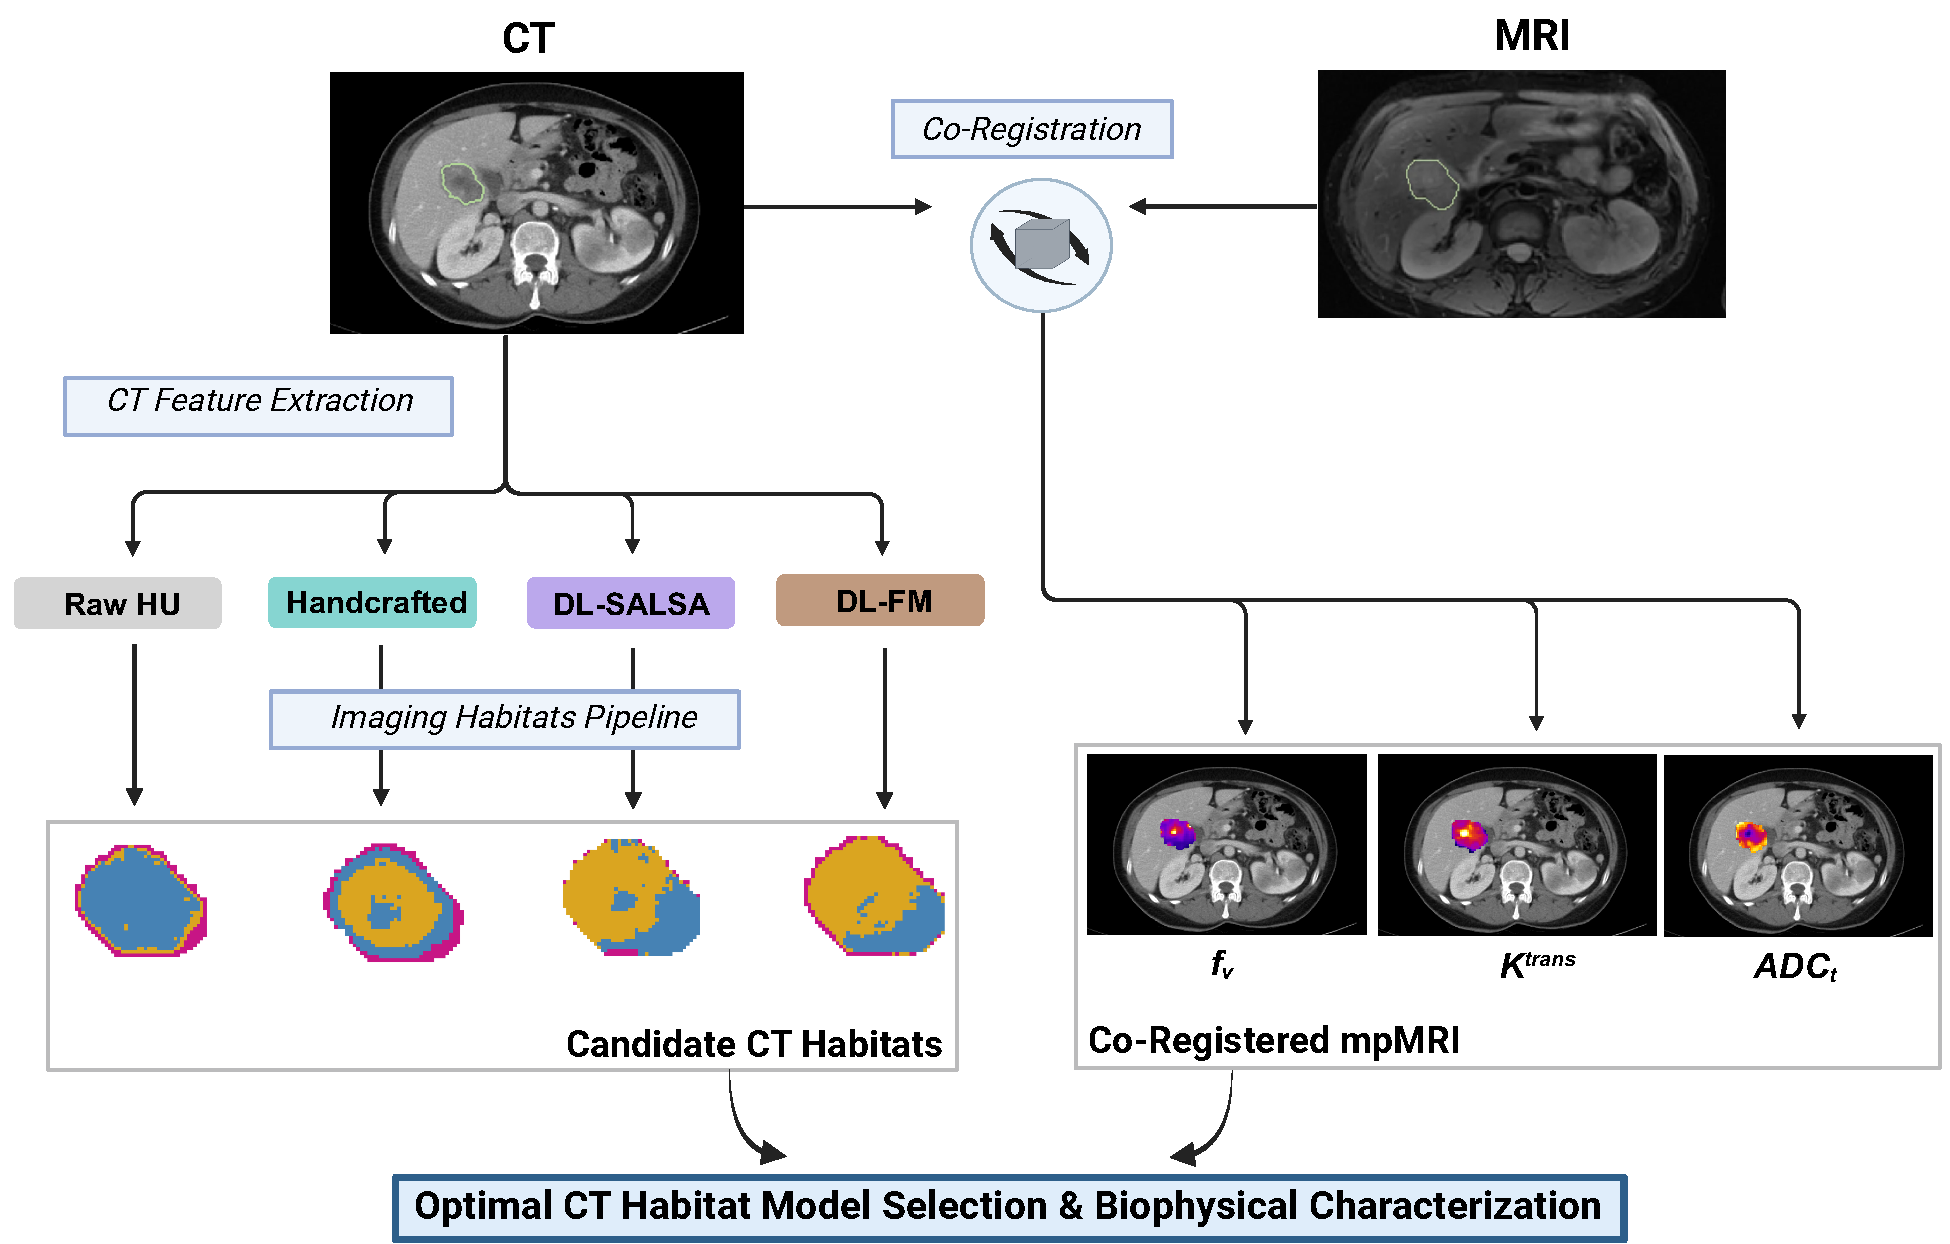
\includegraphics[width=0.95\textwidth]{fig_7_1.pdf}
\caption{Schematic of the mpMRI-anchored CT habitat model development.
CT and MRI scans from the PREDICT cohort were co-registered to T2w
space. Four voxelwise CT feature representations---Raw HU, Handcrafted
Radiomics, DL-SALSA, and DL-FM---were extracted and processed through
the imaging habitats pipeline to generate candidate habitat maps.
Co-registered mpMRI maps (including vascular fraction, $f_v$; capillary
permeability, $K^{trans}$; and tissue apparent diffusion coefficient, $ADC_t$)
provided biophysical reference for model selection. The optimal CT
habitat model was selected based on its ability to spatially separate
tissue properties reflecting cellularity and vascularity (with the three
mpMRI maps shown: ADCt, Ktrans and fv), and further characterized using
additional mpMRI maps. Created with BioRender.com.}
\label{fig:7.1}
\end{figure}

\subsection{CT-mpMRI Co-Registration}\label{ct-mpmri-co-registration}

To enable voxelwise comparison between CT{} and mpMRI, all images were
spatially co-registered to the T2-weighted image, which served as the
fixed reference. This required three registration pipelines: CT{}→T2w,
DWI→T2w, and GRE→T2w. We followed

Images were cropped to a tumor-centered bounding box (5--7 mm margin)
and resampled to 2×2×2 mm isotropic resolution prior to registration.
Registration was performed using NiftyReg in sequential stages: rigid,
affine, then deformable B-spline if alignment improved. Quality was
assessed by Dice similarity coefficient (DSC) between the T2w tumor mask
and the warped mask; the transformation yielding the highest DSC was
retained. Full methodological details are provided in Annex C.

\subsection{CT Feature Extraction}\label{ct-feature-extraction}

Four CT{} representations were evaluated:

\begin{itemize}
\item
  \textbf{Raw Hounsfield units.} The original portal-venous phase CT{}
  images, serving as baseline.
\item
  \textbf{Handcrafted radiomics features.} Voxelwise texture features
  computed using PyRadiomics, based on the 26 precise features
  identified in Chapter 6 (see Section 6.3.2). To avoid clustering on
  redundant information, we removed highly correlated features (Spearman
  \textbar ρ\textbar{} ≥ 0.80), retaining 6 non-redundant features: 10th
  percentile intensity, GLDM dependence entropy, GLDM small dependence
  high gray level emphasis, GLRLM gray level non-uniformity, GLRLM run
  length non-uniformity, and NGTDM coarseness. Correlation analysis is
  detailed in Annex C.
\item
  \textbf{Deep learning features from a liver tumro segmentation model
  (DL-SALSA).} Activations from the penultimate decoder layer of SALSA,
  a 3D nnU-Net trained for liver tumor segmentation (Balaguer-Montero et
  al., 2025).
\item
  \textbf{Deep learning features from a foundation model (DL-FM).}
  Activations from a SegResEncoder foundation model pretrained on
  diverse CT{} datasets using self-supervised learning (Pai et al.,
  2025).
\end{itemize}

All CT{} images were resampled to 1×1×1 mm isotropic resolution prior to
feature extraction. For biological evaluation, the resulting habitat
maps were warped to the T2w reference space (2×2×2 mm) using
nearest-neighbor interpolation.

\subsection{CT Habitat Model Development}\label{ct-habitat-model-development}

\subsubsection{\texorpdfstring{\textbf{7.2.4.1 Clustering
Configuration}}{7.2.4.1 Clustering Configuration}}\label{clustering-configuration}

Habitats were computed using the imaging habitats pipeline described in
Section 5.4, with standard preprocessing: features with high
right-skewness (\textgreater1.0) were log-transformed; all features were
then standardized to zero mean and unit variance. Clustering followed
the two-stage hybrid approach: local GMM clustering within each tumor,
followed by meta-clustering of local centroids to define global
prototypes. The number of habitats was set to K=3, based on the
hypothesis that CT{}-derived clusters could correspond to the dominant
histological compartments of colorectal liver metastases: viable tumor,
necrosis, and fibrosis. The fitted scaler and global prototypes were
saved, enabling application to new data without retraining.

\subsubsection{\texorpdfstring{\textbf{7.2.4.2 CT}{} \textbf{Habitat
Model
Selection}}{7.2.4.2 CT Habitat Model Selection}}\label{ct-habitat-model-selection}

To select the optimal CT{} representation, we evaluated how well each
feature set produced habitats that separate \emph{biologically} distinct
tissue, using the co-registered mpMRI maps as reference. Specifically,
we selected the following three:

\begin{itemize}
\item
  \textbf{ADC\textsubscript{t}} (tissue apparent diffusion coefficient):
  a proxy for cellularity
\item
  \textbf{f\textsubscript{v}} (vascular signal fraction): a measure of
  blood volume
\item
  \textbf{K\textsuperscript{trans}} (volume transfer constant): a
  measure of capillary permeability
\end{itemize}

Both fv and Ktrans were included to capture different aspects of tumor
vascularity---structural vascular density fv versus functional leakiness
and perfusion Ktrans.

For each representation, we computed habitats and extracted the median
value of each mpMRI metric within each habitat for each patient. We
aggregated to patient level (N=10) to avoid pseudo-replication. Habitat
separation was assessed using the Friedman test, with
Kendall\textquotesingle s W as effect size (Kendall \& Smith, 1939;
Tomczak \& Tomczak, n.d.) . To summarize performance across the three
metrics, we computed a biophysical separation score defined as the mean
Kendall\textquotesingle s W across ADCt, fv, and Ktrans. The
representation with the highest biophysical separation score was
selected for further validation.

\subsubsection{\texorpdfstring{\textbf{7.2.4.3 Technical
Validation}}{7.2.4.3 Technical Validation}}\label{technical-validation}

Strong biophysical separation could be spurious if the clustering is
unstable. We therefore evaluated:

\begin{itemize}
\item
  \textbf{Initialization stability.} Mean pairwise Adjusted Rand Index
  across 5 random seeds. High ARI indicates the solution is reproducible
  regardless of initialization.
\item
  \textbf{Data stability.} Mean ARI across 30 bootstrap iterations,
  comparing each resampled model to the full-cohort reference. High ARI
  indicates that habitat definitions are not driven by a few patients.
\item
  \textbf{Spatial coherence.} Moran\textquotesingle s I (spatial
  autocorrelation) and surface-area-to-volume ratio. Biologically
  plausible habitats should form contiguous regions, not scattered
  noise.
\end{itemize}

\subsubsection{\texorpdfstring{\textbf{7.2.4.4 Habitat Characterization
with
mpMRI}}{7.2.4.4 Habitat Characterization with mpMRI}}\label{habitat-characterization-with-mpmri}

Having selected the optimal CT{} representation based on biophysical
separation, we characterized the resulting habitats using the full panel
of mpMRI metrics available in the PREDICT cohort.

Our initial hypothesis was that CT{} habitats would correspond to
histologically defined compartments: necrosis, fibrosis, and viable
tumor. The mpMRI characterization served to test this hypothesis and, if
the correspondence proved incomplete, to build an alternative
interpretive framework based on the tissue properties the habitats
actually captured.

For each of the 13 mpMRI maps (\hyperref[_Ref219812935]{Table 5.2}), we
extracted the median value within each habitat for each patient,
following the same aggregation approach used for model selection.
Differences across the three habitats were assessed using the Friedman
test, with Kendall\textquotesingle s W as effect size. Post-hoc pairwise
comparisons used Wilcoxon signed-rank tests with Benjamini-Hochberg
(Benjamini \& Hochberg, 1995) correction for multiple comparisons within
each metric.

\subsection{Histopathological Validation}\label{histopathological-validation}

To assess whether CT{} habitats correspond to histologically defined
tissue compartments, we applied the trained model to the POEM cohort
(Section 5.1.3). Whole-tumor H\&E sections were digitized and annotated
for viable tumor, necrosis, and fibrosis using a supervised pixel
classifier in QuPath (Bankhead et al., 2017), trained on regions
delineated by the author of this thesis, based on an experienced
pathologist's guidance. Automated annotations were reviewed by the
pathologist for quality assurance. We then performed two experiments:

\begin{itemize}
\item
  \textbf{Qualitative spatial correspondence.} Direct voxel-to-voxel
  co-registration between CT{} and histology was not feasible. We
  therefore evaluated correspondence qualitatively, comparing the
  spatial distribution of CT{} habitats with the architecture visible on
  annotated histology sections.
\item
  \textbf{Correlation with histological tissue percentages}. As an
  exploratory analysis, we computed Spearman correlations between
  whole-tumor habitat proportions and whole-tumor tissue percentages.
\end{itemize}

The primary goal was not to establish quantitative agreement---which
would require spatial co-registration and larger samples---but to
confirm that CT{} habitats exhibit spatial organization consistent with
known histological architecture: viable tumor rims surrounding necrotic
or fibrotic cores.

\section{Results}\label{results-1}

\subsection{Handcrafted Radiomics Yields the Most Biologically Coherent CT Habitats}\label{handcrafted-radiomics-yields-the-most-biologically-coherent-ct-habitats}

\textbf{Co-registration quality.} We first assessed the quality of the
three registration pipelines required for voxelwise CT{}--mpMRI
comparison. The majority of registrations used rigid transformations; no
deformable registration was required. Across 42 tumors, the DWI-to-T2w
registration achieved the highest alignment (median DSC = 0.79, IQR:
0.71--0.84), followed by GRE-to-T2w (median DSC = 0.76, IQR: 0.66--0.85)
and CT{}-to-T2w (median DSC = 0.70, IQR: 0.65--0.78).

\textbf{CT}{} \textbf{Habitat Model Selection.} We compared the four
CT{} representations by their ability to produce habitats that separate
the three pre-specified mpMRI metrics: tissue ADC (cellularity proxy),
vascular fraction (fv), and perfusion (Ktrans).
\hyperref[_Ref219821967]{Figure 7.2} shows examples of CT{} habitats
with the four feature sets. \hyperref[_Ref219821259]{Table 7.1}
summarizes the results.

Handcrafted radiomics achieved the highest biophysical separation score
(mean W = 0.45), driven by strong effects for vascular fraction (W =
0.67, p = 0.005) and perfusion (W = 0.52, p = 0.018). Raw HU showed
moderate separation for cellularity (W = 0.31) but failed to distinguish
vascular phenotypes. DL-SALSA performed moderately on vascular metrics;
DL-FM showed no significant separation on any metric.

Notably, none of the representations achieved strong separation on ADCt,
our primary cellularity proxy. This suggested that CT{} habitats capture
vascular rather than cellular heterogeneity---a finding we examine in
detail in Section 7.3.2.

\textbar{} Comparison of candidate CT{} feature representations

\begin{longtable}[]{@{}
  >{\centering\arraybackslash}p{(\linewidth - 14\tabcolsep) * \real{0.1841}}
  >{\centering\arraybackslash}p{(\linewidth - 14\tabcolsep) * \real{0.0651}}
  >{\centering\arraybackslash}p{(\linewidth - 14\tabcolsep) * \real{0.1189}}
  >{\centering\arraybackslash}p{(\linewidth - 14\tabcolsep) * \real{0.0912}}
  >{\centering\arraybackslash}p{(\linewidth - 14\tabcolsep) * \real{0.1390}}
  >{\centering\arraybackslash}p{(\linewidth - 14\tabcolsep) * \real{0.1227}}
  >{\centering\arraybackslash}p{(\linewidth - 14\tabcolsep) * \real{0.1073}}
  >{\centering\arraybackslash}p{(\linewidth - 14\tabcolsep) * \real{0.1563}}@{}}
\caption{*p \textless{} 0.05 after Bonferroni correction. W =
Kendall\textquotesingle s W effect size.}\tabularnewline
\toprule\noalign{}
\multirow{2}{=}{\centering\arraybackslash \begin{minipage}[b]{\linewidth}\centering
\end{minipage}} &
\multicolumn{2}{>{\centering\arraybackslash}p{(\linewidth - 14\tabcolsep) * \real{0.1841} + 2\tabcolsep}}{%
\begin{minipage}[b]{\linewidth}\centering
\textbf{ADCt}
\end{minipage}} &
\multicolumn{2}{>{\centering\arraybackslash}p{(\linewidth - 14\tabcolsep) * \real{0.2301} + 2\tabcolsep}}{%
\begin{minipage}[b]{\linewidth}\centering
\textbf{Vascular Fraction}
\end{minipage}} &
\multicolumn{2}{>{\centering\arraybackslash}p{(\linewidth - 14\tabcolsep) * \real{0.2300} + 2\tabcolsep}}{%
\begin{minipage}[b]{\linewidth}\centering
\textbf{Ktrans}
\end{minipage}} &
\multirow{2}{=}{\centering\arraybackslash \begin{minipage}[b]{\linewidth}\centering
\textbf{Biophysical Score}
\end{minipage}} \\
& \begin{minipage}[b]{\linewidth}\centering
W
\end{minipage} & \begin{minipage}[b]{\linewidth}\centering
P-value
\end{minipage} & \begin{minipage}[b]{\linewidth}\centering
W
\end{minipage} & \begin{minipage}[b]{\linewidth}\centering
P-value
\end{minipage} & \begin{minipage}[b]{\linewidth}\centering
W
\end{minipage} & \begin{minipage}[b]{\linewidth}\centering
P-value
\end{minipage} \\
\midrule\noalign{}
\endfirsthead
\toprule\noalign{}
\multirow{2}{=}{\centering\arraybackslash \begin{minipage}[b]{\linewidth}\centering
\end{minipage}} &
\multicolumn{2}{>{\centering\arraybackslash}p{(\linewidth - 14\tabcolsep) * \real{0.1841} + 2\tabcolsep}}{%
\begin{minipage}[b]{\linewidth}\centering
\textbf{ADCt}
\end{minipage}} &
\multicolumn{2}{>{\centering\arraybackslash}p{(\linewidth - 14\tabcolsep) * \real{0.2301} + 2\tabcolsep}}{%
\begin{minipage}[b]{\linewidth}\centering
\textbf{Vascular Fraction}
\end{minipage}} &
\multicolumn{2}{>{\centering\arraybackslash}p{(\linewidth - 14\tabcolsep) * \real{0.2300} + 2\tabcolsep}}{%
\begin{minipage}[b]{\linewidth}\centering
\textbf{Ktrans}
\end{minipage}} &
\multirow{2}{=}{\centering\arraybackslash \begin{minipage}[b]{\linewidth}\centering
\textbf{Biophysical Score}
\end{minipage}} \\
& \begin{minipage}[b]{\linewidth}\centering
W
\end{minipage} & \begin{minipage}[b]{\linewidth}\centering
P-value
\end{minipage} & \begin{minipage}[b]{\linewidth}\centering
W
\end{minipage} & \begin{minipage}[b]{\linewidth}\centering
P-value
\end{minipage} & \begin{minipage}[b]{\linewidth}\centering
W
\end{minipage} & \begin{minipage}[b]{\linewidth}\centering
P-value
\end{minipage} \\
\midrule\noalign{}
\endhead
\bottomrule\noalign{}
\endlastfoot
\begin{minipage}[t]{\linewidth}\centering
\begin{quote}
Raw HU
\end{quote}
\end{minipage} & 0.31 & 0.2928 & 0.12 & 0.4894 & 0.04 & 0.6703 &
0.1567 \\
\begin{minipage}[t]{\linewidth}\centering
\begin{quote}
Handcrafted
\end{quote}
\end{minipage} & 0.16 & 0.3281 & 0.67 & 0.0053* & 0.52 & 0.0055* &
0.4500 \\
\begin{minipage}[t]{\linewidth}\centering
\begin{quote}
DL-SALSA
\end{quote}
\end{minipage} & 0.1481 & 0.3808 & 0.4815 & 0.0853 & 0.3457 & 0.0446* &
0.3251 \\
\begin{minipage}[t]{\linewidth}\centering
\begin{quote}
DL-FM
\end{quote}
\end{minipage} & 0.13 & 0.4429 & 0.19 & 0.3889 & 0.13 & 0.2725 &
0.1500 \\
\end{longtable}

To assess whether the three-habitat solution was optimal for the
selected representation, we performed post-hoc sensitivity analyses with
K=2 and K=4. The K=3 solution provided the best balance between
biological interpretability and cluster stability; K=2 merged
biologically distinct vascular phenotypes, while K=4 introduced a
habitat with unstable membership across bootstrap iterations. Results
are detailed in Annex C.

\textbf{Technical validation.} All representations demonstrated high
initialization stability (ARI \textgreater{} 0.96), indicating that the
clustering solution was reproducible regardless of random seed. However,
spatial coherence differed substantially. Handcrafted features produced
spatially contiguous habitats (Moran\textquotesingle s I ≈ 0.80), while
DL-SALSA and DL-FM produced fragmented, "salt-and-pepper" patterns with
low spatial autocorrelation. Full technical validation results are
reported in Annex C.

Based on these findings, handcrafted radiomics was selected as the final
CT{} habitat model.

\begin{figure}[htbp]
\centering
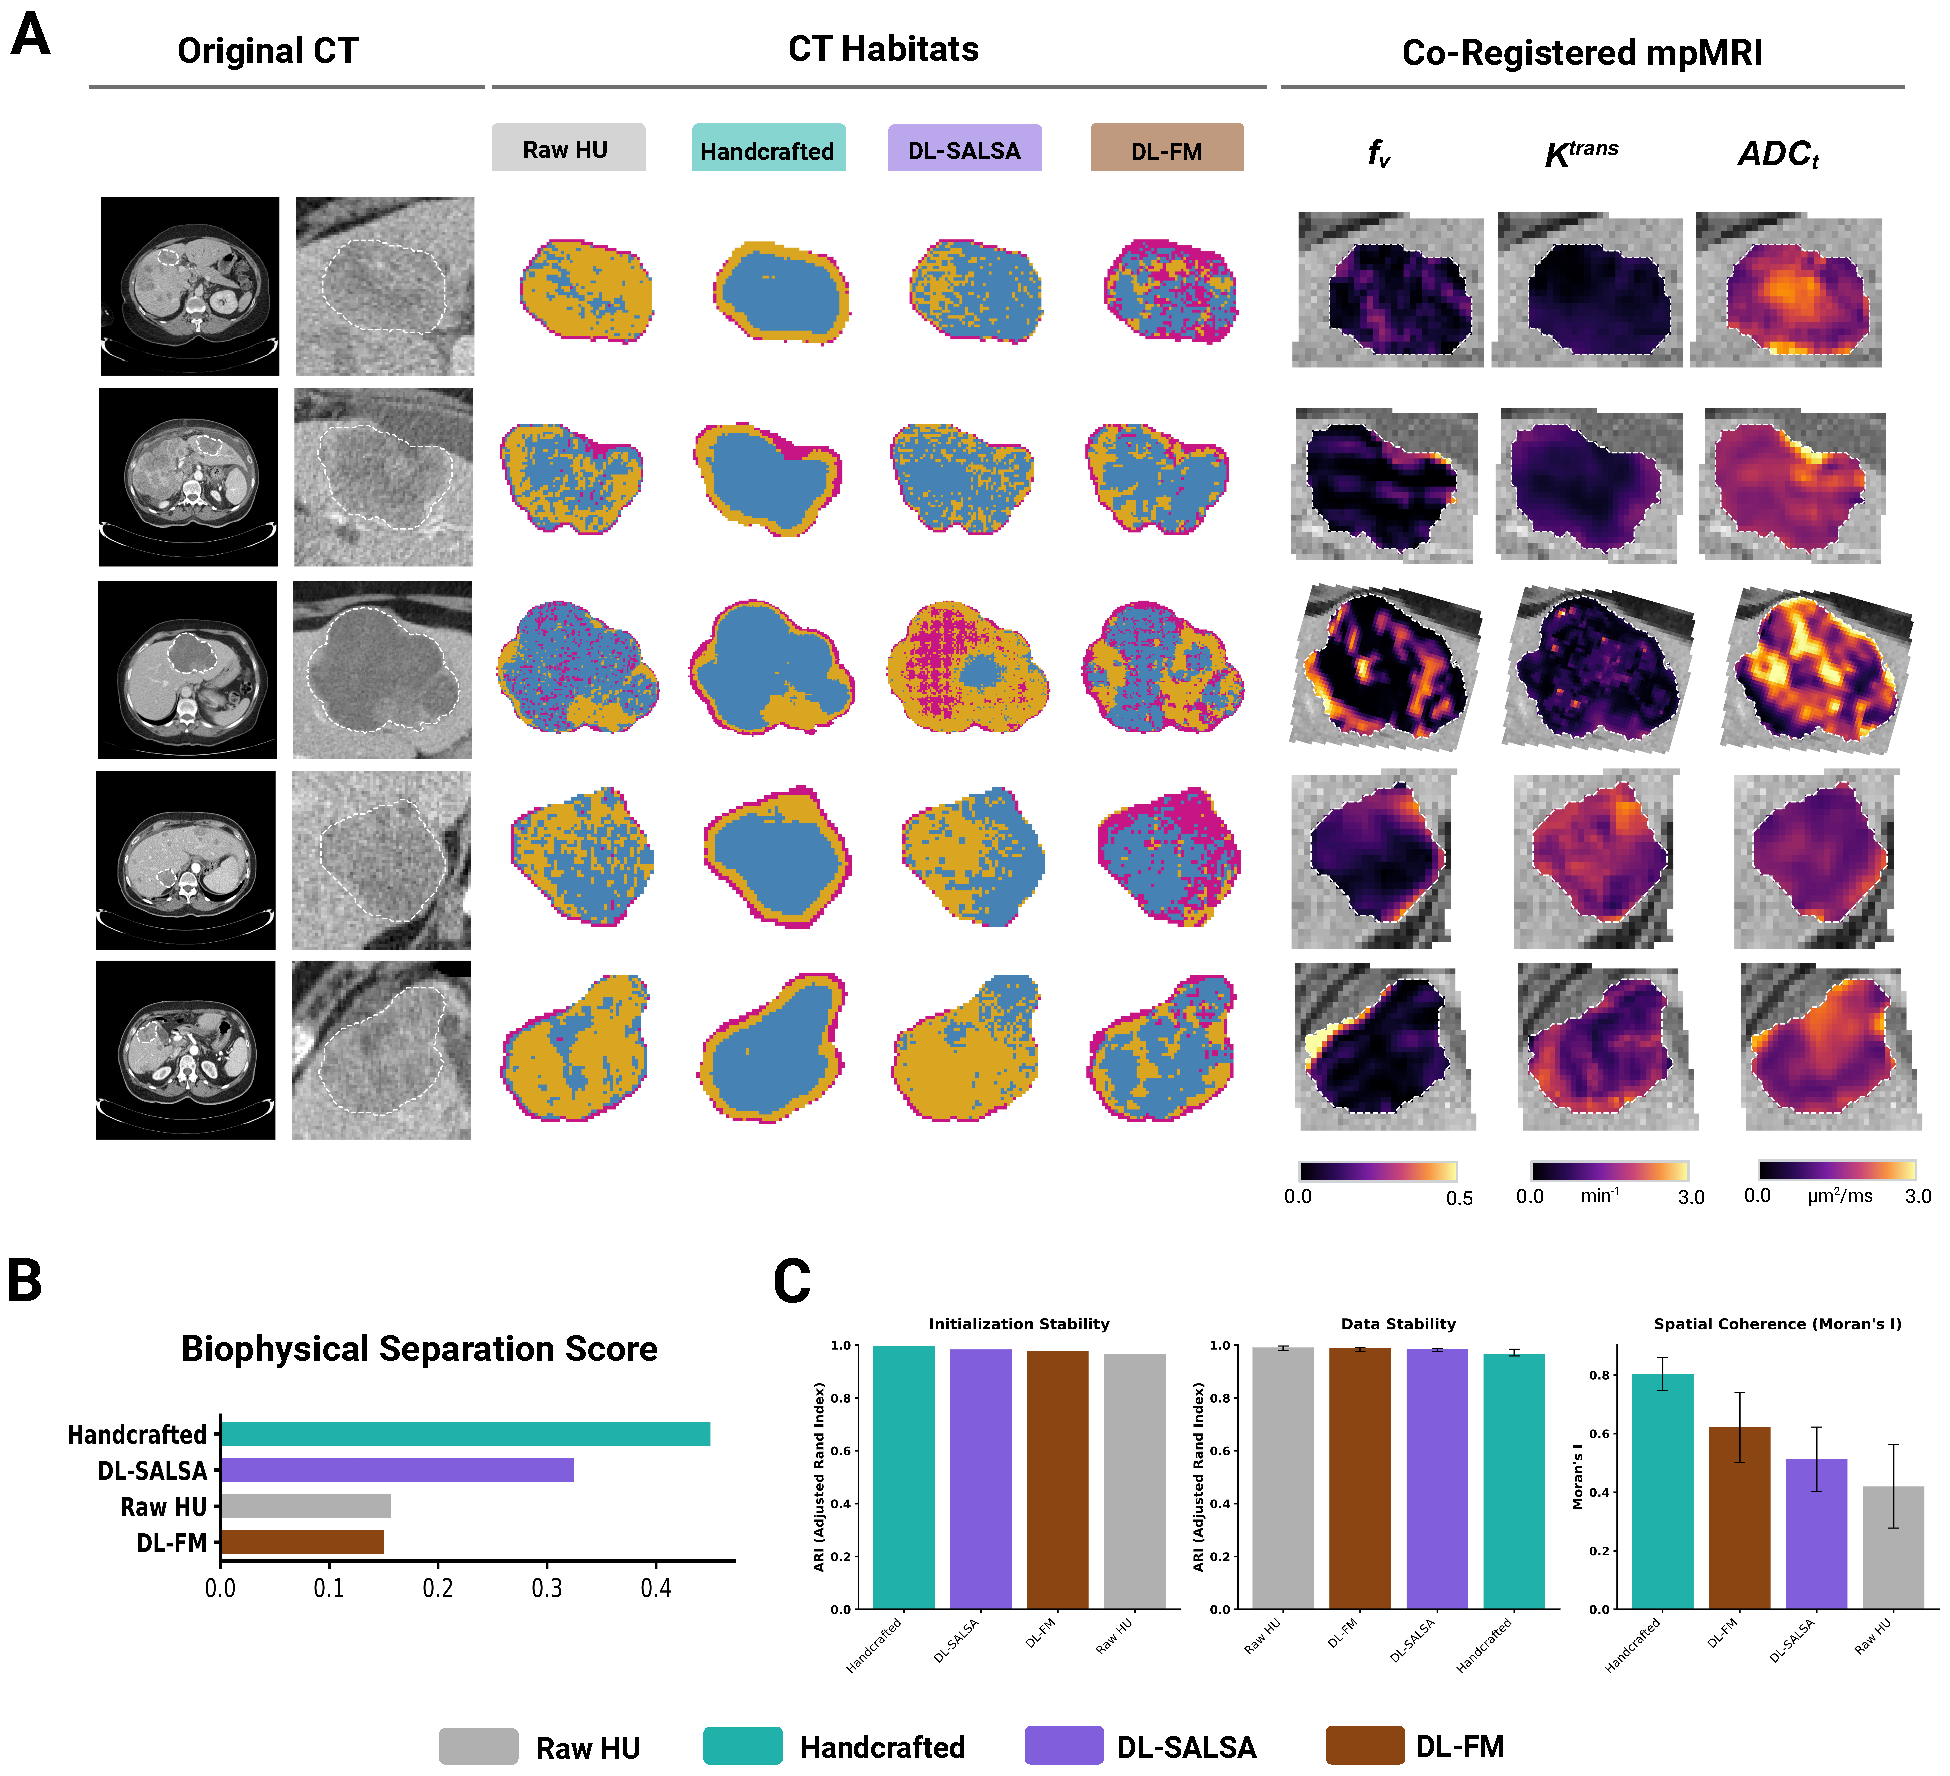
\includegraphics[width=0.95\textwidth]{fig_7_2.pdf}
\caption{Selection of the optimal CT representation.
\textbf{(A)} Representative habitat maps for a single tumor generated by
the four candidate representations (Raw HU, Handcrafted Radiomics,
DL-SALSA, DL-FM), alongside reference mpMRI maps (ADCt, fv, Ktrans).
\textbf{(B)} Biophysical separation performance
(Kendall's W) for each representation across the three
pre-specified mpMRI metrics. Handcrafted radiomics achieved the highest
separation on vascular metrics (fv, Ktrans) but not on cellularity
(ADCt). \textbf{(C)} Technical stability metrics: initialization
stability (ARI across seeds), data stability (bootstrap ARI), and
spatial coherence (Moran's I).}
\label{fig:7.2}
\end{figure}

\subsection{CT Habitats Capture Distinct Vascular and Cellular Phenotypes}\label{ct-habitats-capture-distinct-vascular-and-cellular-phenotypes}

We characterized the three habitats using 13 mpMRI metrics to test
whether they corresponded to the hypothesized histological
compartments---necrosis, fibrosis, and viable tumor
(\hyperref[_Ref219821277]{Table 7.2}). \hyperref[_Ref219821980]{Figure
7.3} shows boxplots for the eight metrics with significant differences
across habitats, plus two cellularity-related metrics (fin, ADCt). Full
results with pairwise significance tests are available in Annex C.

\textbar{} CT{} Habitat Characterization with mpMRI metrics

\begin{longtable}[]{@{}
  >{\centering\arraybackslash}p{(\linewidth - 14\tabcolsep) * \real{0.0649}}
  >{\centering\arraybackslash}p{(\linewidth - 14\tabcolsep) * \real{0.2053}}
  >{\centering\arraybackslash}p{(\linewidth - 14\tabcolsep) * \real{0.1460}}
  >{\centering\arraybackslash}p{(\linewidth - 14\tabcolsep) * \real{0.1196}}
  >{\centering\arraybackslash}p{(\linewidth - 14\tabcolsep) * \real{0.1196}}
  >{\centering\arraybackslash}p{(\linewidth - 14\tabcolsep) * \real{0.1196}}
  >{\centering\arraybackslash}p{(\linewidth - 14\tabcolsep) * \real{0.1124}}
  >{\centering\arraybackslash}p{(\linewidth - 14\tabcolsep) * \real{0.1127}}@{}}
\caption{Patient-level median values for 13 mpMRI-derived biophysical
parameters across the three CT{} habitats (N = 10 patients, 42 tumors).
Vascular parameters (fv, Ktrans, ADCv) show a gradient from H1 to H3;
cellular parameters (ADCt, fin, CD) peak in H2. Significance assessed
using Friedman test with Benjamini-Hochberg correction; effect size
reported as Kendall\textquotesingle s W. BH = Benjamini-Hochberg
correction for multiple comparisons across metrics. W =
Kendall\textquotesingle s W coefficient of concordance (effect size). *p
\textless{} 0.05, **p \textless{} 0.01.}\tabularnewline
\toprule\noalign{}
\multicolumn{2}{@{}>{\centering\arraybackslash}p{(\linewidth - 14\tabcolsep) * \real{0.2702} + 2\tabcolsep}}{%
\multirow{2}{=}{\centering\arraybackslash \begin{minipage}[b]{\linewidth}\centering
\textbf{mpMRI metric}
\end{minipage}}} &
\multirow{2}{=}{\centering\arraybackslash \begin{minipage}[b]{\linewidth}\centering
\textbf{Units}
\end{minipage}} &
\multicolumn{3}{>{\centering\arraybackslash}p{(\linewidth - 14\tabcolsep) * \real{0.3587} + 4\tabcolsep}}{%
\begin{minipage}[b]{\linewidth}\centering
\textbf{Habitats (medians)}
\end{minipage}} &
\multirow{2}{=}{\centering\arraybackslash \begin{minipage}[b]{\linewidth}\centering
\textbf{p-value (BH)}
\end{minipage}} &
\multirow{2}{=}{\centering\arraybackslash \begin{minipage}[b]{\linewidth}\centering
\textbf{Effect Size (W)}
\end{minipage}} \\
& & & \begin{minipage}[b]{\linewidth}\centering
\textbf{H1}
\end{minipage} & \begin{minipage}[b]{\linewidth}\centering
\textbf{H2}
\end{minipage} & \begin{minipage}[b]{\linewidth}\centering
\textbf{H3}
\end{minipage} \\
\midrule\noalign{}
\endfirsthead
\toprule\noalign{}
\multicolumn{2}{@{}>{\centering\arraybackslash}p{(\linewidth - 14\tabcolsep) * \real{0.2702} + 2\tabcolsep}}{%
\multirow{2}{=}{\centering\arraybackslash \begin{minipage}[b]{\linewidth}\centering
\textbf{mpMRI metric}
\end{minipage}}} &
\multirow{2}{=}{\centering\arraybackslash \begin{minipage}[b]{\linewidth}\centering
\textbf{Units}
\end{minipage}} &
\multicolumn{3}{>{\centering\arraybackslash}p{(\linewidth - 14\tabcolsep) * \real{0.3587} + 4\tabcolsep}}{%
\begin{minipage}[b]{\linewidth}\centering
\textbf{Habitats (medians)}
\end{minipage}} &
\multirow{2}{=}{\centering\arraybackslash \begin{minipage}[b]{\linewidth}\centering
\textbf{p-value (BH)}
\end{minipage}} &
\multirow{2}{=}{\centering\arraybackslash \begin{minipage}[b]{\linewidth}\centering
\textbf{Effect Size (W)}
\end{minipage}} \\
& & & \begin{minipage}[b]{\linewidth}\centering
\textbf{H1}
\end{minipage} & \begin{minipage}[b]{\linewidth}\centering
\textbf{H2}
\end{minipage} & \begin{minipage}[b]{\linewidth}\centering
\textbf{H3}
\end{minipage} \\
\midrule\noalign{}
\endhead
\bottomrule\noalign{}
\endlastfoot
ADCₜ & Tissue ADC & μm²/ms & 1.45 & 1.3 & 1.36 & 0.328 & 0.16 \\
ADCᵥ & Vascular ADC & μm²/ms & 16.6 & 16.8 & 17.6 & 0.044* & 0.39 \\
Kₜ & Tissue kurtosis excess & Dimensionless & 0.75 & 0.69 & 0.7 & 0.587
& 0.07 \\
\textbf{fᵥ} & \textbf{Vascular signal fraction} & Normalized & 0.068 &
0.081 & 0.112 & 0.005** & 0.67 \\
T₂ₜ & Tissue T₂ & ms & 81.4 & 100.8 & 82.9 & 0.726 & 0.04 \\
\textbf{D₀} & \textbf{Intrinsic diffusivity} & μm²/ms & 37.5 & 54.1 &
71.6 & 0.001** & 0.84 \\
vCS & Volume-weighted cell size & μm & 24 & 23.6 & 23.9 & 0.529 &
0.09 \\
fᵢₙ & Intracellular fraction & Normalized & 0.46 & 0.5 & 0.48 & 0.113 &
0.28 \\
CD & Cell density & x10\textsuperscript{3} Cells/mm³ & 51.2 & 56.8 &
53.6 & 0.529 & 0.09 \\
\textbf{T₁} & \textbf{T₁} & ms & 1063 & 945 & 911 & 0.019* & 0.49 \\
\textbf{T2\textsuperscript{*}} & \textbf{T2\textsuperscript{*}} & ms &
27.5 & 26.5 & 23.7 & 0.001** & 0.84 \\
\textbf{Kᵗʳᵃⁿˢ} & \textbf{Capillary permeability} & min⁻¹ & 0.41 & 0.52
& 0.51 & 0.018* & 0.52 \\
vₑ & Extracellular-extravascular volume & Normalized & 0.66 & 0.73 &
0.74 & 0.741 & 0.03 \\
\end{longtable}

Vascular parameters showed consistent gradients across habitats.
Vascular fraction (fv) increased monotonically from H1 to H3 (0.068 →
0.112; W = 0.67, p = 0.005), as did vascular ADC. Relaxation times (T2*,
T1) decreased in parallel, consistent with increased blood content and
contrast uptake. However, capillary permeability (Ktrans) did not follow
this gradient---it was highest in H2 (0.52 min⁻¹), not H3 (0.51 min⁻¹),
with both elevated relative to H1 (W = 0.52, p = 0.018). If H3
represented angiogenic tumor tissue, we would expect it to show the
highest Ktrans, since tumor neovessels are typically leaky. The
combination of high fv but moderate Ktrans in H3 suggests partial volume
effects at the tumor-liver interface, where voxels mix tumor tissue with
adjacent normal liver parenchyma---which has mature, less permeable
vasculature.

Cellular parameters showed a different pattern. Metrics related to
cellularity did not follow a simple gradient---instead, H2 emerged as
the most cellular habitat. Tissue ADC was lowest in H2 (1.30 µm²/ms;
pairwise p = 0.029 vs H1), indicating more restricted diffusion.
Intracellular fraction (fin), cell density (CD), and cell size (vCS)
pointed in the same direction: H2 contains the most densely packed
cells. H1, by contrast, showed low-moderate cellularity consistent with
necrotic or fibrotic tissue; H3 showed intermediate values.

\begin{figure}[htbp]
\centering
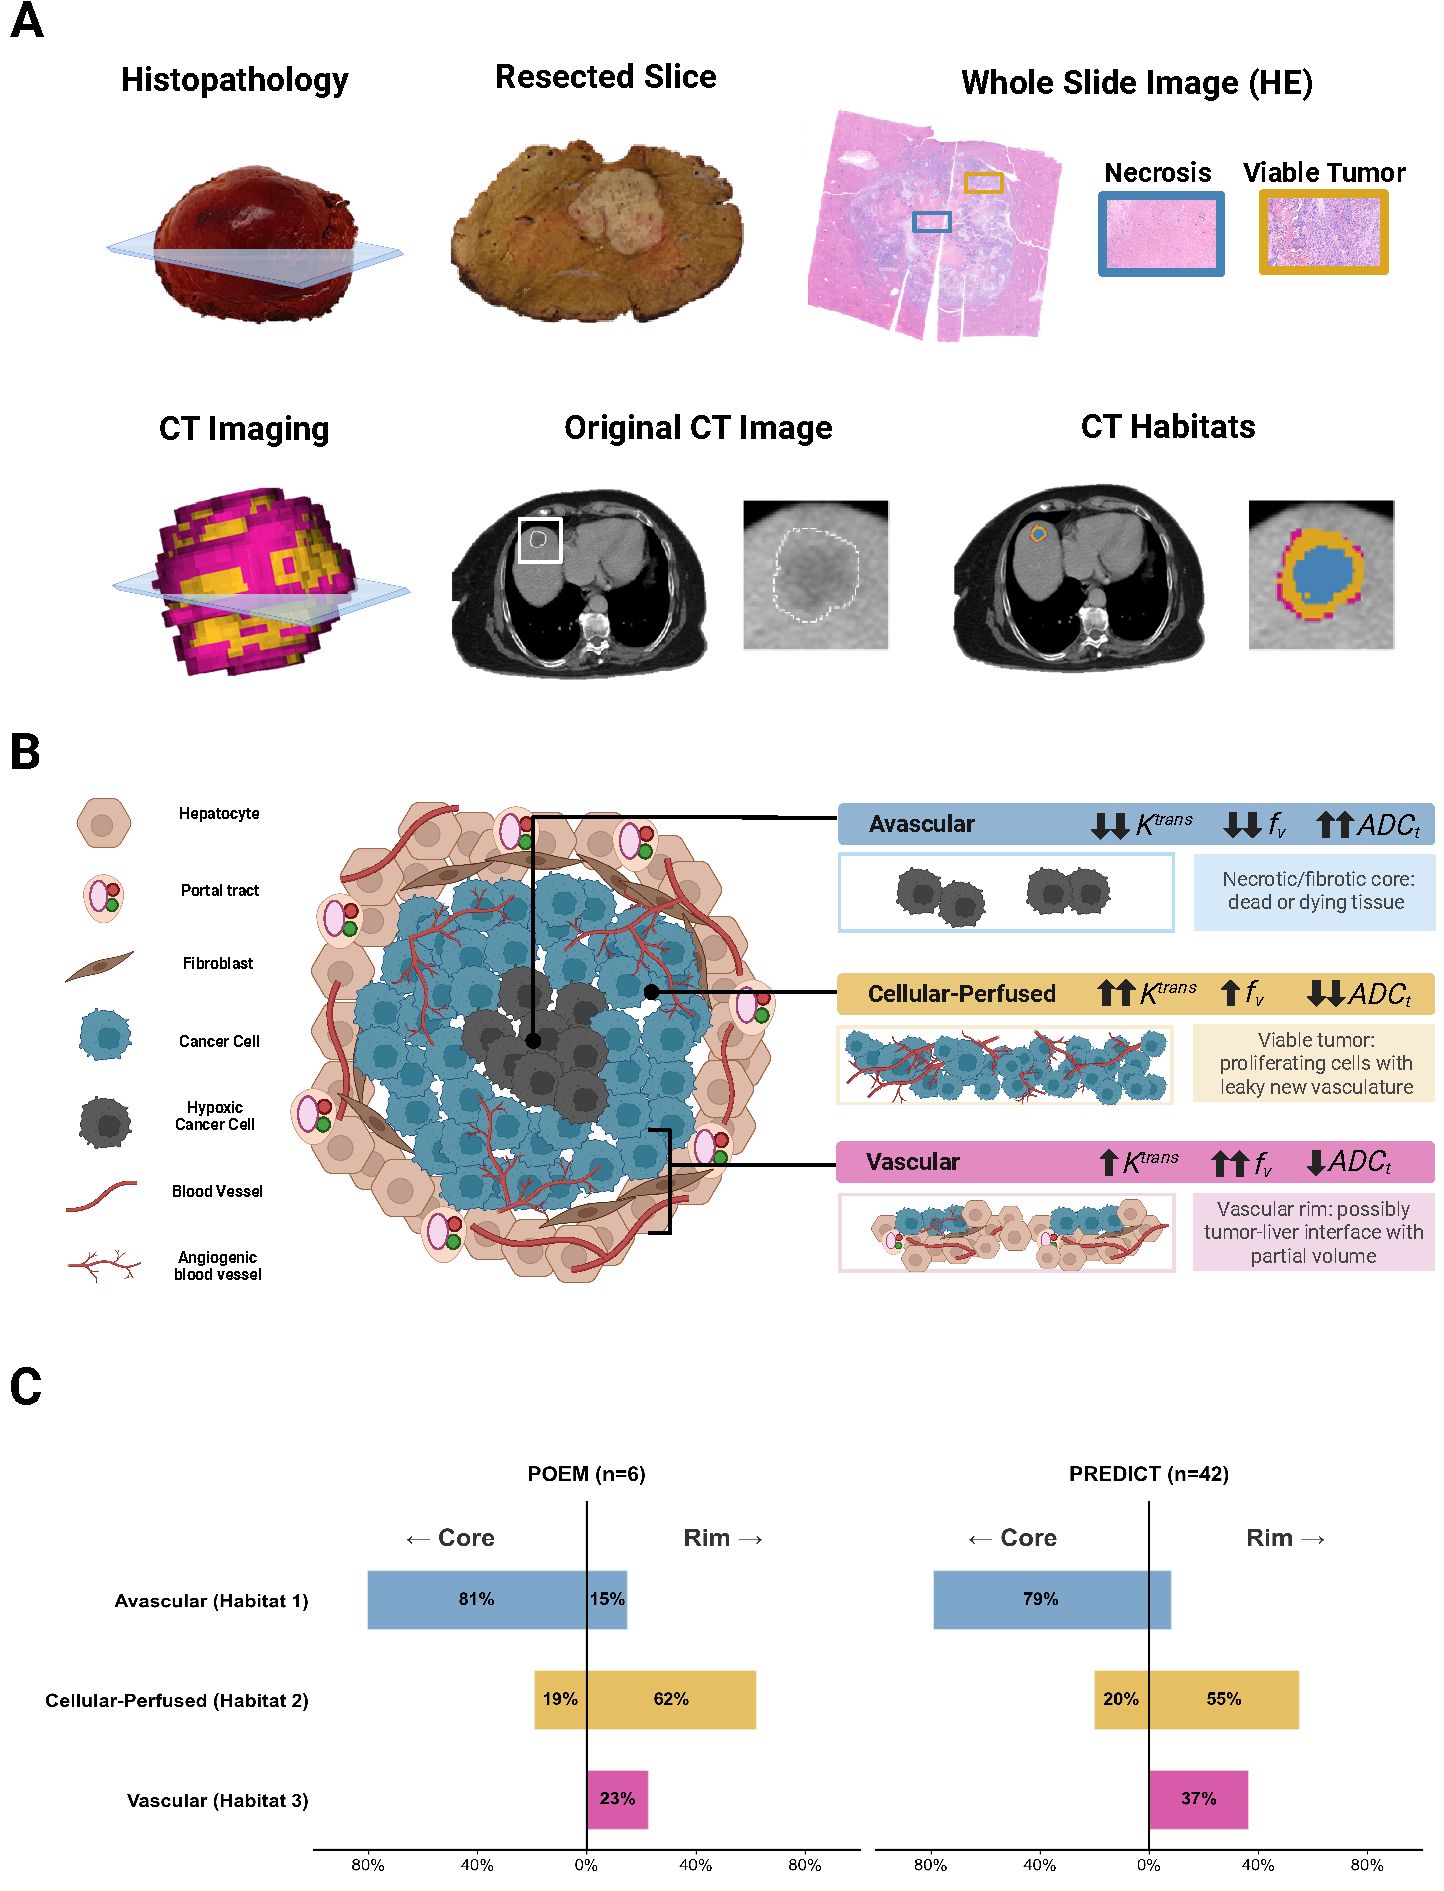
\includegraphics[width=0.95\textwidth]{fig_7_4.pdf}
\caption{Biophysical characterization of CT habitats using mpMRI.
Distribution of eight mpMRI metrics across the three CT habitats (H1:
blue, H2: yellow, H3: pink). Vascular parameters (fv, Ktrans, ADCv, D0)
show gradients from H1 to H3. Cellular parameters (ADCt, fin) show H2 as
the most cellular habitat. Boxplots show patient-level medians (N = 10).
Brackets indicate significant pairwise comparisons (Wilcoxon,
BH-corrected): *p $<$ 0.05, **p $<$ 0.01.}
\label{fig:7.4}
\end{figure}

Based on these profiles, we propose the following biological
interpretation:

\begin{itemize}
\item
  \textbf{Habiat 1: Avascular.} Low vascular fraction, low permeability,
  low-moderate cellularity. Likely contains necrosis, fibrosis, or
  both---CT{} cannot distinguish between them.
\item
  \textbf{Habitat 2: Cellular-Perfused.} Intermediate vascular fraction,
  highest capillary permeability, highest cellularity. Consistent with
  actively proliferating tumor tissue: densely packed viable cells with
  leaky neovessels.
\item
  \textbf{Habitat 3: Vascular.} Highest vascular fraction, moderate
  permeability, moderate cellularity. May capture the tumor-liver
  interface with partial volume from normal liver parenchyma, or a
  vascular-dominant tumor compartment.
\end{itemize}

CT{} habitats thus reflect two aspects of tumor heterogeneity: a
vascular gradient (H1 → H3) and a cellularity peak (H2). The model
distinguishes viable, proliferative tumor (H2) from both the avascular
core (H1) and the vascular interface zone (H3).

\subsection{Spatial Architecture and Histopathological Validation}\label{spatial-architecture-and-histopathologial-validation}

\textbf{Qualitative spatial correspondence.} We applied the trained CT{}
habitat model to the POEM cohort (n = 6) to assess correspondence with
whole-tumor histology. Resected specimens displayed the architecture
characteristic of colorectal liver metastases: central regions of
necrosis and fibrosis surrounded by viable tumor at the periphery
(\hyperref[_Ref219822008]{Figure 7.4}A). CT{} habitat maps captured this
organization---H1 (Avascular) localized to tumor cores, coinciding
mostly with histologically annotated necrosis, while H2
(Cellular-Perfused) and H3 (Vascular) predominated at the periphery,
corresponding to viable tumor margins (\hyperref[_Ref219822008]{Figure
7.4}B).

To quantify this spatial organization, we computed habitat proportions
separately for the tumor rim (2mm outer shell) and core (interior)
across both cohorts (N = 48 tumors: 6 POEM, 42 PREDICT;
\hyperref[_Ref219822008]{Figure 7.4}C). H1 dominated the core (79.4\% ±
2.9\%) but was largely absent from the rim (9.0\% ± 2.3\%). H3 was
concentrated in the rim (35.0\% ± 1.5\%) and virtually absent from the
core (0.4\% ± 0.2\%). H2 showed intermediate localization, enriched in
the rim (56.0\% ± 2.5\%) compared to the core (20.2\% ± 2.9\%). This
pattern was consistent across cohorts: in POEM, cores were 80.5\% H1; in
PREDICT, 79.2\% H1. H3 was absent from POEM cores entirely and
near-absent from PREDICT cores (0.4\%).

\textbf{Correlation with histological tissue percentages}. As an
exploratory analysis, we computed Spearman correlations between
whole-tumor habitat proportions and histological tissue percentages.
Correlations were weak and non-significant (Annex C), reflecting the
scale mismatch between voxel-level imaging and microscopic histology, as
well as CT{}\textquotesingle s inability to distinguish necrosis from
fibrosis within the avascular compartment.

\begin{figure}[htbp]
\centering
\includegraphics[width=0.95\textwidth]{fig_7_3.png}
\caption{Spatial architecture and histopathological validation of CT habitats.
\textbf{(A)} Schematic representation of habitat organization in
colorectal liver metastases. H1 (Avascular, blue) localizes to the tumor
core; H2 (Cellular-Perfused, yellow) represents viable proliferating
tumor; H3 (Vascular, pink) localizes to the periphery at the tumor-liver
interface. \textbf{(B)} Habitat proportions in whole tumor, rim (2mm
outer shell), and core (interior) across both cohorts (POEM n=6, PREDICT
n=42). H1 dominates the core ($\sim$80\%); H2 and H3 dominate
the rim. \textbf{(C)} Representative case from the POEM cohort showing
correspondence between CT habitats and whole-tumor histology. Left:
CT slice with habitat overlay. Right: H\&E section. H1 coincides with
necrotic/fibrotic regions (blue); H2 corresponds to viable tumor at the
periphery (yellow).}
\label{fig:7.3}
\end{figure}

\section{Discussion}\label{discussion-1}

Habitat imaging offers a framework for quantifying intratumor
heterogeneity, but most studies cluster voxels without establishing what
the resulting regions represent biologically. In this chapter, we
addressed this gap by developing an mpMRI-anchored framework for CT{}
habitat discovery. We also addressed a question that has not yet been
studied: which CT{} representation produces the most biologically
coherent habitats? Using co-registered mpMRI as a proxy for tissue
cellularity and vascularity, we compared four CT{} representations and
selected the one whose habitats best separated biologically distinct
tissue phenotypes. We then validated the spatial organization of these
habitats against whole-tumor histopathology.

Handcrafted features outperformed deep learning embeddings for habitat
computation. This was unexpected: foundation models trained on large
CT{} datasets encode rich information, and one might assume they would
produce superior results. However, for unsupervised voxelwise
clustering, stability and spatial coherence matter more than
representational capacity. Deep learning features produced fragmented
patterns while handcrafted features produced contiguous regions aligned
with biological gradients. We note that we did not fine-tune the
foundation model or task-specific embeddings for this application---with
domain-specific optimization, learned representations might perform
better. In Section 9.3. we discuss further the use of handcrafted
features in the era of deep learning.

The mpMRI characterization showed that CT{} habitats mostly reflect
vascular architecture. This is not surprising given that we used
contrast-enhanced portal-venous phase CT{}, where signal intensity
directly reflects contrast uptake and thus tissue perfusion. Our
interpretation of the three habitats was: avascular tissue (H1) with low
fv/Ktrans; a cellular-perfused habitat (H2) towards the rim with highest
Ktrans and celullarity indicating possible viable cancer, and finally a
vascular rim (H3) with highest fv and moderate-high Ktrans. The
fv/Ktrans dissociation in H3 has a plausible explanation: high vascular
fraction but moderate permeability is consistent with the tumor-liver
interface, where voxels mix tumor with normal liver parenchyma that has
mature, less leaky vessels.

The spatial analysis confirmed biological plausibility. Across 48 tumors
from two independent cohorts, H1 dominated tumor cores
(\textasciitilde80\%) while H2 and H3 were enriched at the rim (56\% and
35\%, respectively). This architecture---avascular interior,
vascularized periphery---matches the known histology of colorectal liver
metastases, where viable tumor surrounds a necrotic or fibrotic core
{[}Poultsides et al., 2012; Van den Eynden et al., 2013{]}. Our initial
hypothesis---that CT{} habitats would map onto necrosis, fibrosis, and
viable tumor as discrete categories---was not fully supported. CT{}
reliably separates vascularized from avascular tissue, but within the
avascular core it cannot distinguish necrosis from fibrosis. Both are
hypovascular, lack contrast enhancement, and exhibit similar texture on
portal-venous imaging.

This study presented several limitations. The first one and most
important: habitat labels represent the dominant phenotype for each
voxel. In practice, each voxel (which has an average size of one cubic
millimeter) contains several tissue phenotypes at once. The GMM
clustering assigns each voxel a probability distribution across all
three habitats and we report the maximum-probability assignment. This
discretization loses information---a voxel with 40\% probability for H1
and 35\% for H2 is assigned to H1. Despite this inherent uncertainty,
the spatial segregation is clear: avascular tissue dominates the core,
vascular tissue dominates the rim.

Moreover, sample sizes were small (N = 10 PREDICT, N = 6 POEM),
reflecting the difficulty of acquiring co-registered multimodal imaging
and whole-tumor histology. CT{}-mpMRI registration introduces
uncertainty that propagates into habitat analyses although our median
accuracy (DSC 0.70--0.79) compares favorably with recent benchmarks
{[}Demir et al., 2025{]}. The biological interpretation of H3 as
tumor-liver interface is plausible but not proven---alternative
explanations such as a stromal-rich compartment cannot be excluded.
Finally, histopathological validation was qualitative since voxel-wise
co-registration between CT{} and histology was not feasible.

Despite these limitations, the findings have practical relevance. CT{}
is widely available, reproducible, and already part of standard
oncologic care. If CT{} habitats can stratify patients by tumor vascular
architecture, they could inform treatment decisions without additional
imaging. The distinction between vascularized and avascular compartments
is clinically meaningful: vascularized tissue is more likely to respond
to systemic therapy, while avascular cores may indicate resistance.
Whether habitat-derived metrics predict treatment response or survival
is tested in Chapter 8.

\section{Summary}\label{summary-1}

We developed and validated an mpMRI-anchored CT{} habitat model for
colorectal liver metastases. The central question was whether CT{}
habitats can capture the dominant tissue phenotypes of these tumors.
Using co-registered multiparametric MRI as biological reference and
whole-tumor histopathology for validation, we found that CT{} habitats
reflect vascular architecture---but not discrete histological
categories.

\textbf{Key Points:}

\begin{itemize}
\item
  Handcrafted radiomics features yield the most biologically coherent
  habitats. Comparing four CT{} representations (raw HU, handcrafted
  radiomics, DL-SALSA, DL-FM), handcrafted texture features produced
  habitats with the strongest separation of mpMRI-derived vascular
  parameters and the highest spatial coherence.
\item
  CT{} habitats capture vascular heterogeneity, not discrete
  histological compartments. The three habitats represent an avascular
  core (H1), a cellular-perfused zone with leaky neovessels (H2), and a
  vascular rim likely reflecting the tumor-liver interface (H3). CT{}
  cannot distinguish necrosis from fibrosis within the avascular
  compartment.
\item
  Spatial architecture is biologically plausible and consistent across
  cohorts. H1 dominates tumor cores (\textasciitilde80\%); H2 and H3
  dominate the rim. This organization matches the known histology of
  colorectal liver metastases and was validated against whole-tumor
  histopathology in resected specimens.
\end{itemize}


